\chapter{PHÂN TÍCH CHỨC NĂNG USE CASE}\label{chap3_intro}
\vspace{-40pt}

\section{UC01: Đăng ký}
\begin{usecasetable}
    \textbf{Actor:} & Khách vãng lai. \\ \hline
    \textbf{Mục tiêu:} & Cho phép khách vãng lai tạo tài khoản mới để sử dụng các chức năng dành cho khách hàng. \\ \hline
    \textbf{Mô tả:} & Use Case này cho phép người dùng chưa đăng nhập đăng ký tài khoản mới bằng cách cung cấp các thông tin cần thiết. Hệ thống kiểm tra tính đầy đủ, hợp lệ của thông tin trước khi tạo tài khoản. \\ \hline
    \textbf{Điều kiện trước:} & Người dùng chưa đăng nhập vào hệ thống. \\ \hline
    \textbf{Luồng chính:} & \begin{enumerate}
        \item Người dùng chọn chức năng Đăng ký.
        \item Hệ thống hiển thị biểu mẫu đăng ký.
        \item Người dùng nhập các thông tin cần thiết.
        \item Người dùng gửi thông tin đăng ký.
        \item Hệ thống kiểm tra tính đầy đủ và hợp lệ của thông tin.
        \item Hệ thống kiểm tra tài khoản đã tồn tại hay chưa.
        \item Hệ thống tạo tài khoản mới.
        \item Hệ thống thông báo đăng ký thành công.
    \end{enumerate} \\ \hline
    \textbf{Luồng thay thế / Ngoại lệ:} & \begin{itemize}
        \item Nếu thông tin chưa đầy đủ, hệ thống yêu cầu người dùng bổ sung.
        \item Nếu thông tin không hợp lệ, hệ thống yêu cầu người dùng kiểm tra và nhập lại.
        \item Nếu tài khoản đã tồn tại, hệ thống yêu cầu người dùng sử dụng thông tin khác.
    \end{itemize} \\ \hline
    \textbf{Điều kiện sau:} & Tài khoản mới được tạo thành công. \\ \hline
    \textbf{Quy tắc nghiệp vụ:} & \begin{itemize}
        \item Thông tin đăng ký phải đầy đủ và hợp lệ.
        \item Thông tin định danh tài khoản không được trùng với tài khoản đã tồn tại.
    \end{itemize} \\ \hline
    \textbf{Sơ đồ trình tự:} &  \\ \hline
\end{usecasetable}
\begin{figure}[H]
    \centering
    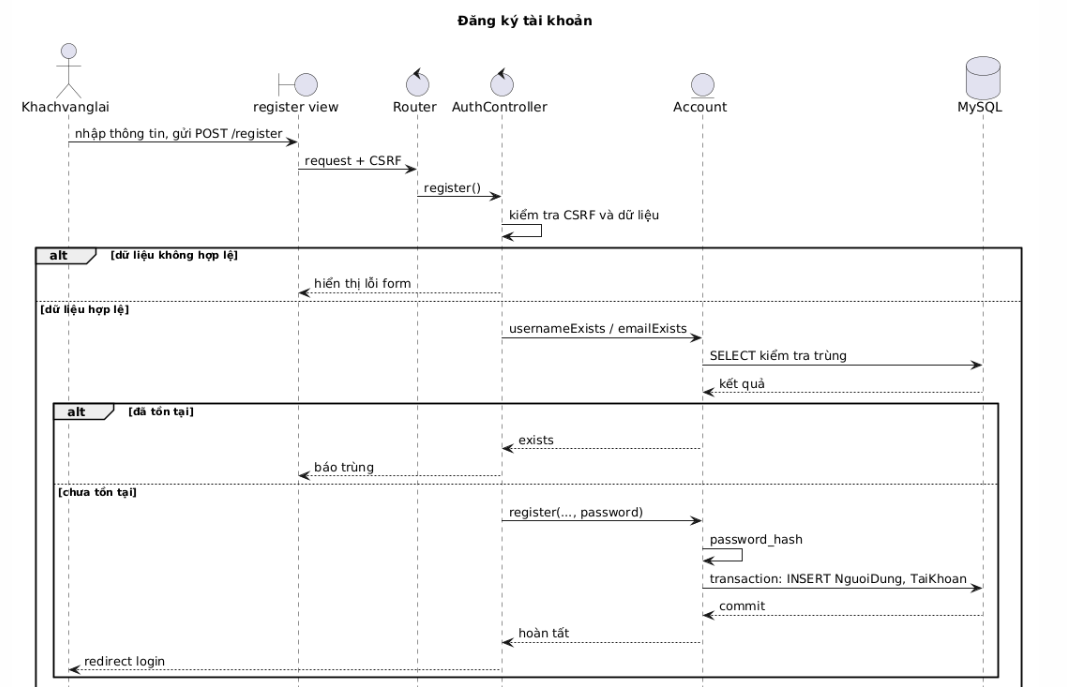
\includegraphics[width=0.9\textwidth, keepaspectratio]{Chapter_3/images_Usecase/đăng ký.png}
    \caption{Sơ đồ trình tự Usecase Đăng ký}
    \label{fig:uc-dang-ky}
\end{figure}

\section{UC02: Đăng nhập}
\begin{usecasetable}
    \textbf{Actor:} & Khách vãng lai, Google Identity. \\ \hline
    \textbf{Mục tiêu:} & Cho phép người dùng xác thực tài khoản và đăng nhập vào hệ thống. \\ \hline
    \textbf{Mô tả:} & Use Case này cho phép người dùng cung cấp thông tin đăng nhập. Hệ thống kiểm tra thông tin xác thực và trạng thái tài khoản trước khi thiết lập trạng thái đăng nhập. \\ \hline
    \textbf{Điều kiện trước:} & Người dùng chưa đăng nhập vào hệ thống. \\ \hline
    \textbf{Luồng chính:} & \begin{enumerate}
        \item Người dùng chọn chức năng Đăng nhập.
        \item Hệ thống hiển thị biểu mẫu đăng nhập bằng tài khoản hệ thống và lựa chọn đăng nhập bằng Google.
        \item Người dùng chọn phương thức đăng nhập. Đối với phương thức đăng nhập bằng tài khoản hệ thống, người dùng nhập tên đăng nhập/email và mật khẩu rồi gửi biểu mẫu.
        \item Hệ thống kiểm tra thông tin đăng nhập hoặc chuyển người dùng đến Google Identity để xác thực.
        \item Khi xác thực qua Google thành công, Google Identity trả thông tin định danh đã xác minh; hệ thống tìm tài khoản Google đã liên kết hoặc tạo tài khoản Khách hàng mới theo quy tắc nghiệp vụ.
        \item Hệ thống kiểm tra trạng thái tài khoản.
        \item Hệ thống thiết lập trạng thái đăng nhập.
        \item Hệ thống thông báo đăng nhập thành công và điều hướng người dùng theo vai trò.
    \end{enumerate} \\ \hline
    \textbf{Luồng thay thế / Ngoại lệ:} & \begin{itemize}
        \item Nếu thông tin đăng nhập chưa đầy đủ, hệ thống yêu cầu người dùng nhập lại.
        \item Nếu tài khoản không tồn tại, hệ thống cho phép người dùng chuyển sang UC01 -- Đăng ký.
        \item Nếu mật khẩu không chính xác, hệ thống yêu cầu người dùng nhập lại.
        \item Nếu người dùng hủy xác thực Google hoặc xác thực không hợp lệ, hệ thống từ chối đăng nhập.
        \item Nếu email Google thuộc tài khoản hiện có nhưng chưa được liên kết, hệ thống yêu cầu người dùng xác thực tài khoản hiện có để liên kết.
        \item Nếu tài khoản ở trạng thái Không còn hoạt động hoặc Bị vô hiệu hóa, hệ thống từ chối đăng nhập.
        \item Nếu không thể thiết lập trạng thái đăng nhập, hệ thống yêu cầu người dùng thực hiện lại.
    \end{itemize} \\ \hline
    \textbf{Điều kiện sau:} & Người dùng được xác thực và đăng nhập thành công. Khách hàng được chuyển đến trang chủ; Quản trị viên được chuyển đến trang tổng quan quản trị. \\ \hline
    \textbf{Quy tắc nghiệp vụ:} & \begin{itemize}
        \item Chỉ tài khoản tồn tại và đang ở trạng thái Hoạt động mới được phép đăng nhập.
        \item Tài khoản mới tạo bằng Google mặc định có vai trò Khách hàng.
        \item Tài khoản Google được liên kết bằng mã định danh ổn định sau khi xác minh chữ ký, đối tượng nhận, thời hạn và trạng thái email.
    \end{itemize} \\ \hline
    \textbf{Sơ đồ trình tự:} &  \\ \hline
\end{usecasetable}
\begin{figure}[H]
    \centering
    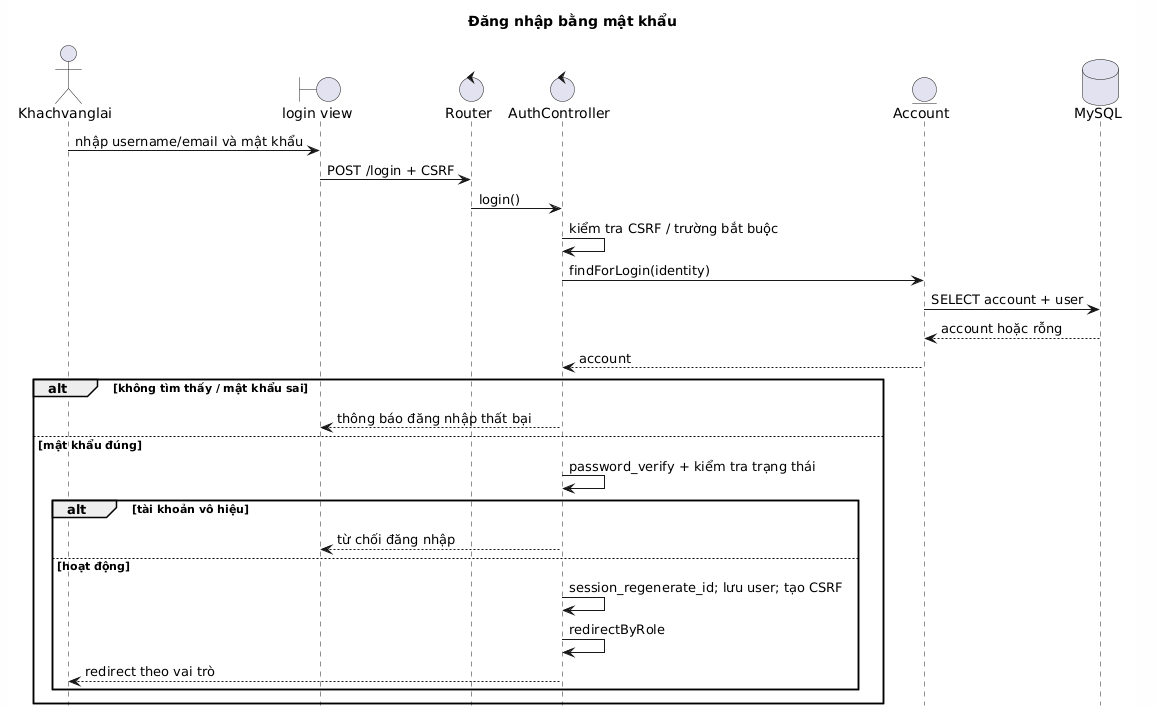
\includegraphics[width=0.9\textwidth, keepaspectratio]{Chapter_3/images_Usecase/Đăng_nhập.png}
    \caption{Sơ đồ trình tự Usecase Đăng nhập}
    \label{fig:uc-dang-nhap}
\end{figure}

\begin{figure}[H]
    \centering
    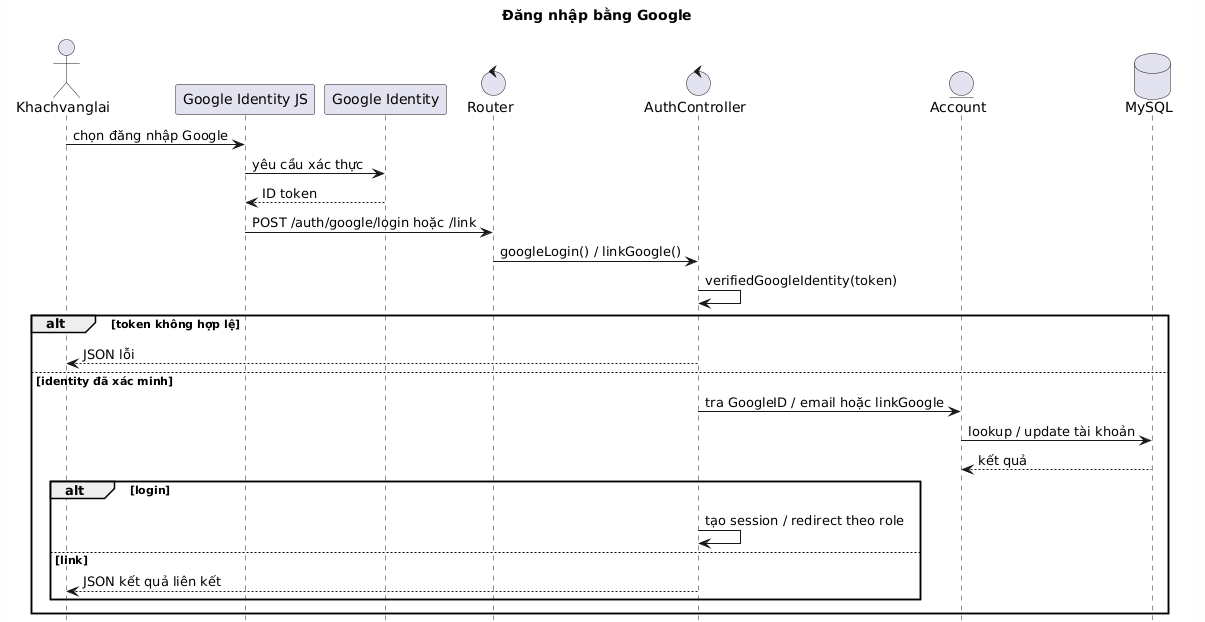
\includegraphics[width=0.9\textwidth, keepaspectratio]{Chapter_3/images_Usecase/loginGoogle.png}
    \caption{Sơ đồ trình tự Usecase Đăng nhập bằng Google}
    \label{fig:uc-dang-nhap-google}
    \end{figure}

\section{UC03: Xem, tìm kiếm và lọc sản phẩm}
\begin{usecasetable}
    \textbf{Actor:} & Khách vãng lai, Khách hàng. \\ \hline
    \textbf{Mục tiêu:} & Cho phép người dùng tra cứu và xem thông tin sản phẩm phù hợp với nhu cầu. \\ \hline
    \textbf{Mô tả:} & Use Case này cho phép người dùng xem danh sách sản phẩm mà không cần đăng nhập. Người dùng có thể tìm kiếm bằng từ khóa, lựa chọn danh mục, lọc theo khoảng giá, thương hiệu hoặc thuộc tính kỹ thuật và xem thông tin chi tiết. \\ \hline
    \textbf{Điều kiện trước:} & Sản phẩm tồn tại và đang được phép hiển thị trên website. \\ \hline
    \textbf{Luồng chính:} & \begin{enumerate}
        \item Người dùng truy cập khu vực hiển thị sản phẩm.
        \item Hệ thống hiển thị danh sách sản phẩm đang kinh doanh.
        \item Người dùng có thể chọn danh mục sản phẩm.
        \item Người dùng có thể nhập từ khóa tìm kiếm.
        \item Người dùng có thể lọc theo loại sản phẩm, thương hiệu, khoảng giá và thuộc tính kỹ thuật được hỗ trợ.
        \item Hệ thống hiển thị giá niêm yết, giá sau giảm và thông tin chương trình giảm giá đang có hiệu lực nếu có.
        \item Hệ thống xử lý yêu cầu và hiển thị kết quả phù hợp.
        \item Người dùng chọn một sản phẩm.
        \item Hệ thống hiển thị tên, hình ảnh, giá, mô tả, thông số kỹ thuật và tình trạng tồn kho.
    \end{enumerate} \\ \hline
    \textbf{Luồng thay thế / Ngoại lệ:} & \begin{itemize}
        \item Nếu không tìm thấy sản phẩm phù hợp, hệ thống hiển thị danh sách kết quả trống.
        \item Sản phẩm ngừng kinh doanh không được hiển thị trong danh sách thông thường.
        \item Sản phẩm hết hàng vẫn có thể hiển thị kèm tình trạng hết hàng.
        \item Nếu chương trình giảm giá hết hạn, hệ thống chỉ hiển thị giá niêm yết.
    \end{itemize} \\ \hline
    \textbf{Điều kiện sau:} & Người dùng nhận được danh sách hoặc thông tin chi tiết sản phẩm. \\ \hline
    \textbf{Quy tắc nghiệp vụ:} & \begin{itemize}
        \item Không yêu cầu đăng nhập để xem, tìm kiếm và lọc sản phẩm.
        \item Chỉ sản phẩm đang được phép kinh doanh mới được hiển thị trong danh sách thông thường.
        \item Giá trị lọc theo loại, thương hiệu và thuộc tính phải lấy từ dữ liệu phân loại đã được Quản trị viên khai báo.
    \end{itemize} \\ \hline
\end{usecasetable}

\section{UC04: Quản lý giỏ hàng}
\begin{usecasetable}
    \textbf{Actor:} & Khách hàng. \\ \hline
    \textbf{Mục tiêu:} & Cho phép khách hàng quản lý các sản phẩm dự định mua. \\ \hline
    \textbf{Mô tả:} & Khách hàng có thể thêm sản phẩm vào giỏ hàng, thay đổi số lượng hoặc xóa sản phẩm không còn nhu cầu mua. Giỏ hàng được quản lý theo tài khoản và được duy trì sau khi đăng xuất và đăng nhập lại. \\ \hline
    \textbf{Điều kiện trước:} & \begin{itemize}
        \item Người dùng đã đăng nhập.
        \item Sản phẩm muốn thêm đang kinh doanh và còn tồn kho.
    \end{itemize} \\ \hline
    \textbf{Luồng chính:} & \begin{enumerate}
        \item Khách hàng chọn sản phẩm và chức năng thêm vào giỏ.
        \item Hệ thống kiểm tra số lượng tồn kho.
        \item Hệ thống cập nhật sản phẩm và số lượng vào giỏ hàng.
        \item Khách hàng truy cập giỏ hàng để xem danh sách.
        \item Khách hàng thay đổi số lượng hoặc xóa sản phẩm.
        \item Hệ thống cập nhật dữ liệu và tính lại tổng tiền.
    \end{enumerate} \\ \hline
    \textbf{Luồng thay thế / Ngoại lệ:} & \begin{itemize}
        \item Nếu khách vãng lai thao tác giỏ hàng, hệ thống chuyển sang trang Đăng nhập UC02.
        \item Nếu số lượng vượt tồn kho, hệ thống không cập nhật giỏ và thông báo lỗi.
        \item Nếu sản phẩm ngừng kinh doanh, hệ thống từ chối thêm.
    \end{itemize} \\ \hline
    \textbf{Điều kiện sau:} & Giỏ hàng của tài khoản được cập nhật trong cơ sở dữ liệu. \\ \hline
    \textbf{Quy tắc nghiệp vụ:} & \begin{itemize}
        \item Số lượng trong giỏ phải lớn hơn 0 và không vượt quá tồn kho.
        \item Không cho phép thêm sản phẩm ngừng kinh doanh.
    \end{itemize} \\ \hline
\end{usecasetable}

\section{UC05: Đặt hàng}
\begin{usecasetable}
    \textbf{Actor:} & Khách hàng. \\ \hline
    \textbf{Mục tiêu:} & Tạo đơn hàng từ các sản phẩm trong giỏ hàng. \\ \hline
    \textbf{Mô tả:} & Khách hàng kiểm tra sản phẩm, số lượng, giá sau giảm, chọn địa chỉ giao hàng, nhập voucher và chọn phương thức thanh toán. Hệ thống kiểm tra lại giá, giảm giá, voucher và tồn kho trước khi tạo đơn ở trạng thái Chờ xác nhận. \\ \hline
    \textbf{Điều kiện trước:} & Khách hàng đã đăng nhập và giỏ hàng có ít nhất một sản phẩm. \\ \hline
    \textbf{Luồng chính:} & \begin{enumerate}
        \item Khách hàng truy cập giỏ hàng.
        \item Khách hàng chọn chức năng Đặt hàng.
        \item Hệ thống hiển thị sản phẩm, giá niêm yết, giá sau giảm và tổng tiền tạm tính.
        \item Khách hàng nhập hoặc chọn thông tin nhận hàng.
        \item Khách hàng có thể nhập mã voucher theo UC18.
        \item Hệ thống kiểm tra voucher và cập nhật số tiền giảm, tổng tiền phải trả.
        \item Khách hàng lựa chọn phương thức thanh toán.
        \item Hệ thống kiểm tra thông tin và tồn kho tại thời điểm đặt hàng.
        \item Khách hàng xác nhận đặt hàng.
        \item Hệ thống tạo đơn hàng ở trạng thái Chờ xác nhận.
    \end{enumerate} \\ \hline
    \textbf{Luồng thay thế / Ngoại lệ:} & Nếu thông tin nhận hàng không hợp lệ, giỏ hàng không còn sản phẩm hợp lệ hoặc voucher không hợp lệ, hệ thống thông báo và yêu cầu khách hàng điều chỉnh. \\ \hline
    \textbf{Điều kiện sau:} & Đơn hàng được tạo ở trạng thái Chờ xác nhận. \\ \hline
    \textbf{Quy tắc nghiệp vụ:} & \begin{itemize}
        \item Không tạo đơn hàng khi giỏ hàng trống.
        \item Đặt hàng và thanh toán là hai nghiệp vụ riêng biệt.
        \item Hệ thống tạm trừ số lượng tồn kho khi đơn hàng được tạo thành công.
        \item Hệ thống tự tính lại giá khuyến mãi và voucher; không tin số tiền giảm do trình duyệt gửi lên.
        \item Tổng tiền, số tiền giảm và voucher được lưu cùng đơn hàng để giữ lịch sử giao dịch.
    \end{itemize} \\ \hline
\end{usecasetable}

\section{UC06: Thanh toán}
\begin{usecasetable}
    \textbf{Actor:} & Khách hàng, Cổng thanh toán. \\ \hline
    \textbf{Mục tiêu:} & Xử lý thanh toán cho đơn hàng. \\ \hline
    \textbf{Mô tả:} & Khách hàng có thể thanh toán khi nhận hàng hoặc thanh toán trực tuyến. COD ghi nhận trạng thái Chưa thanh toán; thanh toán trực tuyến được gửi đến Cổng thanh toán và cập nhật theo kết quả. \\ \hline
    \textbf{Điều kiện trước:} & Đơn hàng đã được tạo, chưa hủy và đang ở trạng thái chưa thanh toán. \\ \hline
    \textbf{Luồng chính:} & \begin{enumerate}
        \item Khách hàng truy cập chức năng thanh toán cho đơn hàng chưa thanh toán.
        \item Hệ thống kiểm tra trạng thái đơn và trạng thái thanh toán.
        \item Hệ thống xác định phương thức đã lựa chọn khi đặt hàng.
        \item Nếu là COD, hệ thống ghi nhận Chưa thanh toán.
        \item Nếu là trực tuyến, hệ thống tạo yêu cầu giao dịch và gửi đến Cổng thanh toán.
        \item Cổng thanh toán xử lý và trả kết quả.
        \item Hệ thống kiểm tra kết quả và cập nhật trạng thái thanh toán.
    \end{enumerate} \\ \hline
    \textbf{Luồng thay thế / Ngoại lệ:} & \begin{itemize}
        \item Giao dịch thất bại hoặc bị hủy, hệ thống giữ trạng thái Chưa thanh toán.
        \item Đơn đã thanh toán hoặc đã hủy không được thanh toán lại.
        \item Không nhận được kết quả hợp lệ thì không cập nhật thành Đã thanh toán.
    \end{itemize} \\ \hline
    \textbf{Điều kiện sau:} & Trạng thái thanh toán được ghi nhận là Chưa thanh toán hoặc Đã thanh toán. \\ \hline
    \textbf{Quy tắc nghiệp vụ:} & \begin{itemize}
        \item Chỉ xác nhận thanh toán trực tuyến khi nhận được kết quả hợp lệ.
        \item Đơn đã thanh toán không được thanh toán lại.
    \end{itemize} \\ \hline
    \textbf{Sơ đồ trình tự:} &  \\ \hline
\end{usecasetable}
\begin{figure}[H]
    \centering
    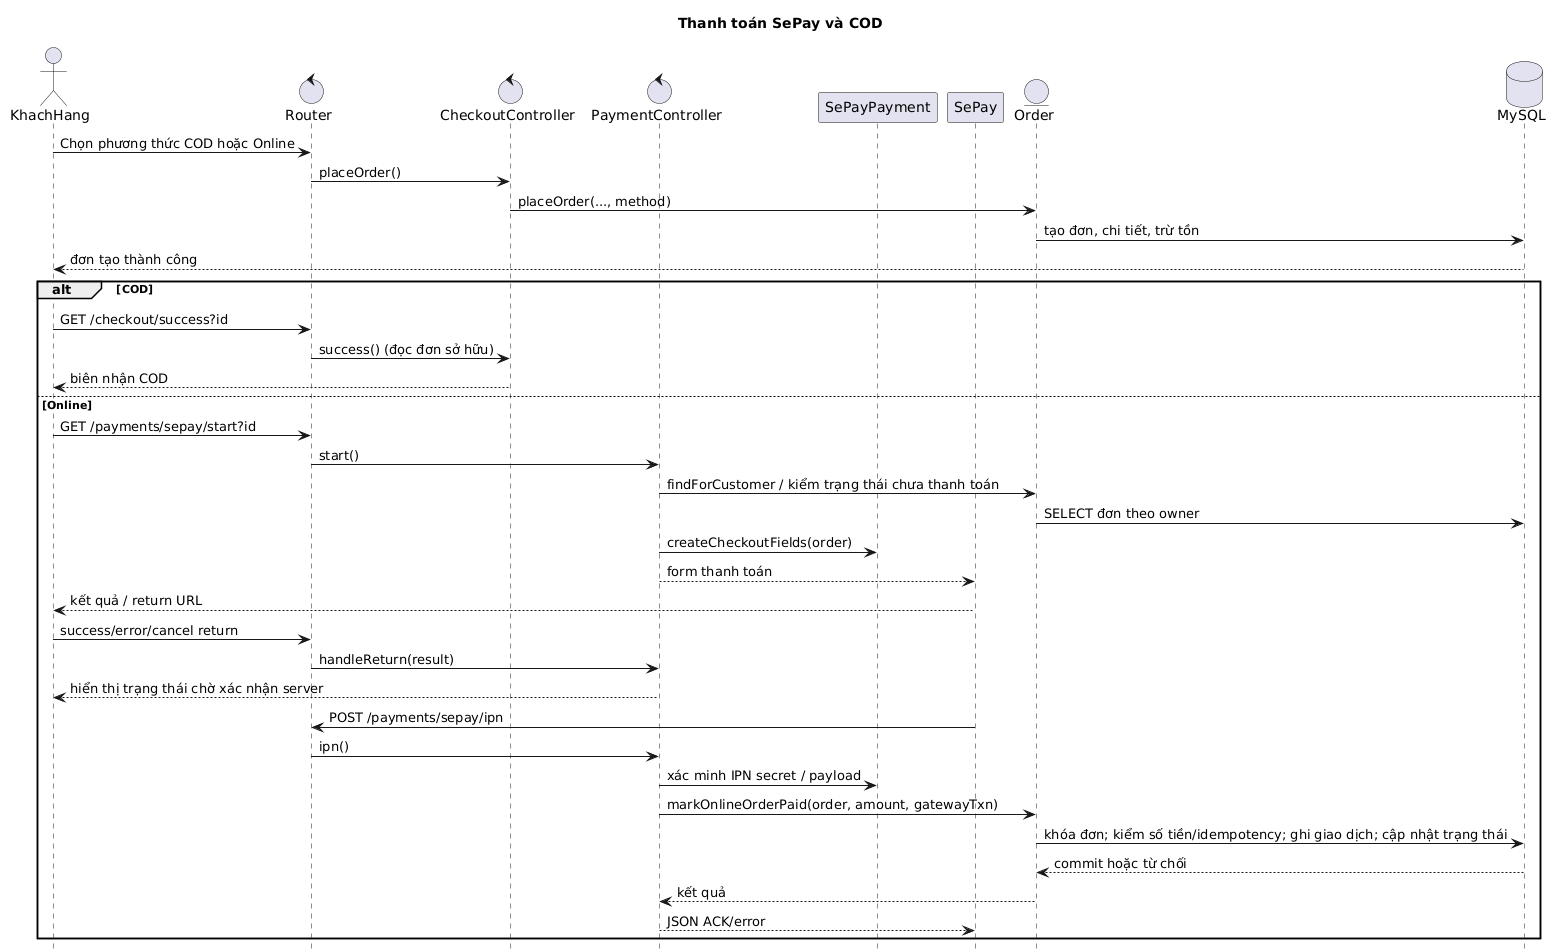
\includegraphics[width=0.9\textwidth, keepaspectratio]{Chapter_3/images_Usecase/Thanh_toán.png}
    \caption{Sơ đồ trình tự Usecase Thanh toán}
    \label{fig:uc-thanh-toan}
    \end{figure}

\section{UC07: Theo dõi và hủy đơn hàng}
\begin{usecasetable}
    \textbf{Actor:} & Khách hàng. \\ \hline
    \textbf{Mục tiêu:} & Cho phép khách hàng theo dõi tình trạng đơn hàng và hủy đơn khi đáp ứng điều kiện. \\ \hline
    \textbf{Mô tả:} & Khách hàng xem danh sách và chi tiết đơn hàng thuộc tài khoản mình, theo dõi trạng thái xử lý và thanh toán. Khách hàng chỉ được hủy khi đơn đang ở trạng thái Chờ xác nhận. \\ \hline
    \textbf{Điều kiện trước:} & \begin{itemize}
        \item Khách hàng đã đăng nhập.
        \item Đơn hàng tồn tại và thuộc tài khoản đang đăng nhập.
    \end{itemize} \\ \hline
    \textbf{Luồng chính:} & \begin{enumerate}
        \item Khách hàng chọn một đơn hàng để xem chi tiết.
        \item Hệ thống hiển thị thông tin đơn, trạng thái xử lý và thanh toán.
        \item Nếu đơn đang ở trạng thái Chờ xác nhận, hệ thống hiển thị chức năng hủy đơn.
        \item Khách hàng chọn hủy đơn.
        \item Hệ thống kiểm tra trạng thái đơn.
        \item Hệ thống cập nhật đơn thành Đã hủy.
        \item Hệ thống thông báo kết quả.
    \end{enumerate} \\ \hline
    \textbf{Luồng thay thế / Ngoại lệ:} & \begin{itemize}
        \item Nếu đơn không thuộc tài khoản, hệ thống từ chối truy cập.
        \item Nếu đơn không còn ở trạng thái Chờ xác nhận, hệ thống không cho phép hủy.
        \item Nếu đơn đã hủy hoặc không tồn tại, hệ thống thông báo trạng thái phù hợp.
    \end{itemize} \\ \hline
    \textbf{Điều kiện sau:} & Thông tin đơn được hiển thị hoặc trạng thái đơn được cập nhật thành Đã hủy. \\ \hline
    \textbf{Quy tắc nghiệp vụ:} & \begin{itemize}
        \item Khách hàng chỉ xem đơn thuộc tài khoản của mình.
        \item Chỉ hủy được đơn ở trạng thái Chờ xác nhận.
        \item Đơn đã Đang chuẩn bị hàng trở đi không được khách hàng tự hủy.
        \item Đơn đã hủy không được hủy lại.
    \end{itemize} \\ \hline
\end{usecasetable}

\section{UC08: Quản lý tài khoản}
\begin{usecasetable}
    \textbf{Actor:} & Khách hàng. \\ \hline
    \textbf{Mục tiêu:} & Cho phép khách hàng quản lý thông tin tài khoản. \\ \hline
    \textbf{Mô tả:} & Khách hàng xem và cập nhật thông tin cá nhân, liên hệ, mật khẩu và sổ địa chỉ giao hàng. Khách hàng có thể lưu nhiều địa chỉ và chọn một địa chỉ khi đặt hàng. \\ \hline
    \textbf{Điều kiện trước:} & Khách hàng đã đăng nhập. \\ \hline
    \textbf{Luồng chính:} & \begin{enumerate}
        \item Khách hàng truy cập thông tin tài khoản.
        \item Hệ thống hiển thị thông tin hiện có.
        \item Khách hàng chỉnh sửa thông tin cá nhân, mật khẩu hoặc địa chỉ giao hàng.
        \item Hệ thống kiểm tra dữ liệu.
        \item Hệ thống lưu thay đổi và gắn địa chỉ với tài khoản.
    \end{enumerate} \\ \hline
    \textbf{Luồng thay thế / Ngoại lệ:} & Nếu dữ liệu không hợp lệ hoặc mật khẩu hiện tại không chính xác, hệ thống không lưu thay đổi. Nếu địa chỉ không thuộc tài khoản, hệ thống từ chối thao tác. \\ \hline
    \textbf{Điều kiện sau:} & Thông tin tài khoản được cập nhật. \\ \hline
    \textbf{Quy tắc nghiệp vụ:} & Một khách hàng có thể lưu nhiều địa chỉ. Địa chỉ đã chụp vào đơn hàng phải được giữ nguyên trong lịch sử khi khách hàng sửa hoặc xóa địa chỉ trong sổ địa chỉ. \\ \hline
\end{usecasetable}

\section{UC09: Quản lý đơn hàng}
\begin{usecasetable}
    \textbf{Actor:} & Nhân viên, Quản trị viên. \\ \hline
    \textbf{Mục tiêu:} & Theo dõi và xử lý các đơn hàng trong hệ thống. \\ \hline
    \textbf{Mô tả:} & Nhân viên và Quản trị viên xem danh sách, kiểm tra thông tin và xử lý đơn hàng theo quyền. Đơn ở trạng thái Chờ xác nhận được kiểm tra thông tin và tồn kho trước khi chuyển sang Đang chuẩn bị hàng. \\ \hline
    \textbf{Phân quyền:} & \begin{itemize}
        \item Nhân viên được xem danh sách, xem chi tiết, kiểm tra tồn kho, xác nhận và cập nhật trạng thái trong phạm vi quyền.
        \item Quản trị viên được xem và quản lý toàn bộ đơn hàng.
    \end{itemize} \\ \hline
    \textbf{Điều kiện trước:} & Nhân viên hoặc Quản trị viên đã đăng nhập và có quyền xử lý đơn hàng. \\ \hline
    \textbf{Luồng chính:} & \begin{enumerate}
        \item Người dùng truy cập danh sách đơn hàng.
        \item Hệ thống kiểm tra quyền và hiển thị đơn theo phạm vi quyền.
        \item Người dùng chọn một đơn để xem chi tiết.
        \item Hệ thống hiển thị thông tin đơn, trạng thái xử lý và thanh toán.
        \item Khi đơn ở trạng thái Chờ xác nhận, người dùng kiểm tra thông tin và tồn kho.
        \item Hệ thống kiểm tra lại trạng thái và tồn kho.
        \item Nếu hợp lệ, người dùng xác nhận đơn.
        \item Hệ thống chuyển đơn sang Đang chuẩn bị hàng.
        \item Người dùng cập nhật trạng thái theo quy trình: Đang chuẩn bị hàng -> Đang giao hàng -> Hoàn thành hoặc Giao hàng thất bại.
        \item Hệ thống lưu thay đổi và thực hiện xử lý liên quan.
    \end{enumerate} \\ \hline
    \textbf{Luồng thay thế / Ngoại lệ:} & \begin{itemize}
        \item Nếu không có quyền, hệ thống từ chối thao tác.
        \item Nếu tồn kho không đáp ứng, hệ thống không cho phép xác nhận.
        \item Nếu đơn đã được xử lý bởi người khác hoặc chuyển trạng thái không hợp lệ, hệ thống từ chối thao tác.
        \item Khi Giao hàng thất bại, tồn kho chỉ được cộng trả lại sau khi xác nhận hàng hoàn về kho.
    \end{itemize} \\ \hline
    \textbf{Điều kiện sau:} & Thông tin và trạng thái đơn được cập nhật theo thao tác hợp lệ. \\ \hline
    \textbf{Quy tắc nghiệp vụ:} & \begin{itemize}
        \item Tồn kho phải được kiểm tra lại tại thời điểm xác nhận.
        \item Không trừ tồn kho lần thứ hai nếu số lượng đã được tạm trừ khi tạo đơn.
        \item Trạng thái phải tuân theo quy trình và không được chuyển tùy ý.
        \item Đơn đã hủy, hoàn thành hoặc giao hàng thất bại không được chuyển sang trạng thái xử lý khác.
    \end{itemize} \\ \hline
\end{usecasetable}

\section{UC10: Kiểm tra tồn kho}
\begin{usecasetable}
    \textbf{Actor:} & Nhân viên. \\ \hline
    \textbf{Mục tiêu:} & Tra cứu số lượng sản phẩm còn trong kho để hỗ trợ xử lý đơn hàng. \\ \hline
    \textbf{Mô tả:} & Nhân viên có thể tìm kiếm hoặc chọn sản phẩm để xem số lượng tồn kho hiện tại. Chức năng này không cho phép tự điều chỉnh kho. \\ \hline
    \textbf{Điều kiện trước:} & Nhân viên đã đăng nhập. \\ \hline
    \textbf{Luồng chính:} & \begin{enumerate}
        \item Nhân viên truy cập chức năng kiểm tra tồn kho.
        \item Nhân viên nhập hoặc chọn sản phẩm.
        \item Hệ thống truy xuất thông tin tồn kho.
        \item Hệ thống hiển thị số lượng hiện có.
    \end{enumerate} \\ \hline
    \textbf{Luồng thay thế / Ngoại lệ:} & Nếu không tìm thấy sản phẩm, hệ thống thông báo. \\ \hline
    \textbf{Điều kiện sau:} & Thông tin tồn kho được hiển thị. \\ \hline
    \textbf{Quy tắc nghiệp vụ:} & Nhân viên chỉ có quyền tra cứu, không được trực tiếp điều chỉnh số lượng tồn kho. \\ \hline
\end{usecasetable}

\section{UC11: Quản lý sản phẩm}
\begin{usecasetable}
    \textbf{Actor:} & Quản trị viên. \\ \hline
    \textbf{Mục tiêu:} & Quản lý thông tin các sản phẩm được kinh doanh. \\ \hline
    \textbf{Mô tả:} & Quản trị viên thêm mới, chỉnh sửa và cập nhật trạng thái kinh doanh của sản phẩm. Thông tin gồm tên, giá niêm yết, hình ảnh, mô tả, danh mục, loại sản phẩm, thương hiệu và thông số kỹ thuật. Giá khuyến mãi được quản lý riêng trong UC16. \\ \hline
    \textbf{Điều kiện trước:} & Quản trị viên đã đăng nhập. \\ \hline
    \textbf{Luồng chính:} & \begin{enumerate}
        \item Quản trị viên truy cập chức năng quản lý sản phẩm.
        \item Hệ thống hiển thị danh sách sản phẩm và thao tác được phép.
        \item Quản trị viên chọn thêm, chỉnh sửa hoặc đổi trạng thái kinh doanh.
        \item Hệ thống hiển thị biểu mẫu phù hợp.
        \item Quản trị viên nhập hoặc cập nhật thông tin sản phẩm.
        \item Quản trị viên gửi biểu mẫu.
        \item Hệ thống kiểm tra dữ liệu bắt buộc, định dạng và ràng buộc.
        \item Hệ thống lưu sản phẩm hoặc cập nhật dữ liệu.
        \item Hệ thống thông báo kết quả.
    \end{enumerate} \\ \hline
    \textbf{Luồng thay thế / Ngoại lệ:} & \begin{itemize}
        \item Nếu dữ liệu thiếu hoặc không hợp lệ, hệ thống yêu cầu chỉnh sửa.
        \item Nếu sản phẩm hoặc danh mục không tồn tại, hệ thống từ chối lưu.
        \item Nếu lưu thất bại, dữ liệu sản phẩm hiện có không thay đổi.
        \item Nếu phiên đăng nhập không hợp lệ hoặc không có quyền, hệ thống từ chối thao tác.
    \end{itemize} \\ \hline
    \textbf{Điều kiện sau:} & Thông tin hoặc trạng thái sản phẩm được cập nhật khi thao tác thành công. \\ \hline
    \textbf{Quy tắc nghiệp vụ:} & \begin{itemize}
        \item Sản phẩm chỉ ở trạng thái Đang kinh doanh hoặc Ngừng kinh doanh.
        \item Sản phẩm đã phát sinh trong đơn hàng không được xóa vật lý.
        \item Số lượng tồn kho được quản lý trong UC14.
        \item Giá niêm yết không bị ghi đè bởi giá khuyến mãi.
    \end{itemize} \\ \hline
\end{usecasetable}

\section{UC12: Quản lý danh mục}
\begin{usecasetable}
    \textbf{Actor:} & Quản trị viên. \\ \hline
    \textbf{Mục tiêu:} & Quản lý việc phân loại sản phẩm. \\ \hline
    \textbf{Mô tả:} & Quản trị viên thêm mới, chỉnh sửa hoặc cập nhật trạng thái danh mục. Danh mục kết hợp với loại sản phẩm, thương hiệu và thuộc tính kỹ thuật để hỗ trợ lọc sản phẩm trong UC03. \\ \hline
    \textbf{Điều kiện trước:} & Quản trị viên đã đăng nhập. \\ \hline
    \textbf{Luồng chính:} & \begin{enumerate}
        \item Quản trị viên truy cập chức năng quản lý danh mục.
        \item Hệ thống hiển thị danh sách danh mục.
        \item Quản trị viên chọn thêm, chỉnh sửa hoặc đổi trạng thái.
        \item Hệ thống hiển thị biểu mẫu tương ứng.
        \item Quản trị viên nhập tên, mô tả và thông tin cần cập nhật.
        \item Hệ thống kiểm tra tính đầy đủ, hợp lệ và tính duy nhất.
        \item Hệ thống lưu danh mục hoặc cập nhật trạng thái.
        \item Hệ thống thông báo kết quả.
    \end{enumerate} \\ \hline
    \textbf{Luồng thay thế / Ngoại lệ:} & \begin{itemize}
        \item Nếu tên trùng hoặc dữ liệu không hợp lệ, hệ thống không lưu.
        \item Nếu danh mục còn sản phẩm liên kết, hệ thống không cho xóa vật lý mà hướng dẫn chuyển sang Ngừng kinh doanh.
        \item Nếu danh mục không tồn tại hoặc lưu thất bại, hệ thống thông báo lỗi.
    \end{itemize} \\ \hline
    \textbf{Điều kiện sau:} & Thông tin hoặc trạng thái danh mục được cập nhật khi thành công. \\ \hline
    \textbf{Quy tắc nghiệp vụ:} & \begin{itemize}
        \item Không tạo danh mục trùng lặp.
        \item Danh mục có trạng thái Đang kinh doanh hoặc Ngừng kinh doanh.
        \item Chỉ cho phép xóa cứng danh mục không có sản phẩm liên kết.
    \end{itemize} \\ \hline
\end{usecasetable}

\section{UC13: Quản lý người dùng}
\begin{usecasetable}
    \textbf{Actor:} & Quản trị viên. \\ \hline
    \textbf{Mục tiêu:} & Quản lý tài khoản khách hàng và nhân viên. \\ \hline
    \textbf{Mô tả:} & Quản trị viên xem, tìm kiếm và quản lý trạng thái tài khoản. Tài khoản nhân viên có thể được thêm mới hoặc cập nhật thông tin; tài khoản khách hàng có thể được xem và khóa hoặc mở khóa. \\ \hline
    \textbf{Điều kiện trước:} & Quản trị viên đã đăng nhập. \\ \hline
    \textbf{Luồng chính:} & \begin{enumerate}
        \item Quản trị viên truy cập chức năng quản lý người dùng.
        \item Hệ thống hiển thị danh sách tài khoản.
        \item Quản trị viên tìm kiếm hoặc chọn tài khoản.
        \item Quản trị viên thực hiện thao tác phù hợp với loại tài khoản.
        \item Hệ thống kiểm tra quyền và dữ liệu.
        \item Hệ thống lưu thay đổi.
    \end{enumerate} \\ \hline
    \textbf{Luồng thay thế / Ngoại lệ:} & Nếu dữ liệu không hợp lệ hoặc thao tác không được phép, hệ thống từ chối và thông báo. \\ \hline
    \textbf{Điều kiện sau:} & Thông tin hoặc trạng thái tài khoản được cập nhật. \\ \hline
    \textbf{Quy tắc nghiệp vụ:} & \begin{itemize}
        \item Tài khoản Hoạt động được phép đăng nhập.
        \item Tài khoản Bị vô hiệu hóa không được phép đăng nhập cho đến khi được mở khóa.
        \item Không xóa cứng tài khoản đã liên quan đến dữ liệu giao dịch.
        \item Không được làm mất quyền của tài khoản quản trị cuối cùng.
    \end{itemize} \\ \hline
\end{usecasetable}

\section{UC14: Quản lý kho}
\begin{usecasetable}
    \textbf{Actor:} & Quản trị viên. \\ \hline
    \textbf{Mục tiêu:} & Theo dõi và cập nhật số lượng hàng hóa trong kho. \\ \hline
    \textbf{Mô tả:} & Quản trị viên theo dõi tồn kho và thực hiện nhập hoặc điều chỉnh số lượng sản phẩm khi cần thiết. \\ \hline
    \textbf{Điều kiện trước:} & Quản trị viên đã đăng nhập. \\ \hline
    \textbf{Luồng chính:} & \begin{enumerate}
        \item Quản trị viên truy cập chức năng quản lý kho.
        \item Hệ thống hiển thị thông tin tồn kho.
        \item Quản trị viên chọn sản phẩm cần cập nhật.
        \item Quản trị viên nhập hoặc điều chỉnh số lượng.
        \item Hệ thống kiểm tra dữ liệu.
        \item Hệ thống cập nhật số lượng tồn kho.
    \end{enumerate} \\ \hline
    \textbf{Luồng thay thế / Ngoại lệ:} & Nếu số lượng không hợp lệ hoặc làm tồn kho nhỏ hơn 0, hệ thống từ chối. \\ \hline
    \textbf{Điều kiện sau:} & Số lượng tồn kho được cập nhật. \\ \hline
    \textbf{Quy tắc nghiệp vụ:} & \begin{itemize}
        \item Số lượng tồn kho không được nhỏ hơn 0.
        \item Mọi thay đổi tồn kho phải được kiểm tra trước khi lưu.
        \item Số lượng tồn kho không được cập nhật trực tiếp trong UC11.
        \item Thay đổi tồn kho ghi nhận sản phẩm, số lượng, loại thao tác, người thực hiện và thời gian.
    \end{itemize} \\ \hline
    \textbf{Sơ đồ trình tự:} &  \\ \hline
\end{usecasetable}
\begin{figure}[H]
    \centering
    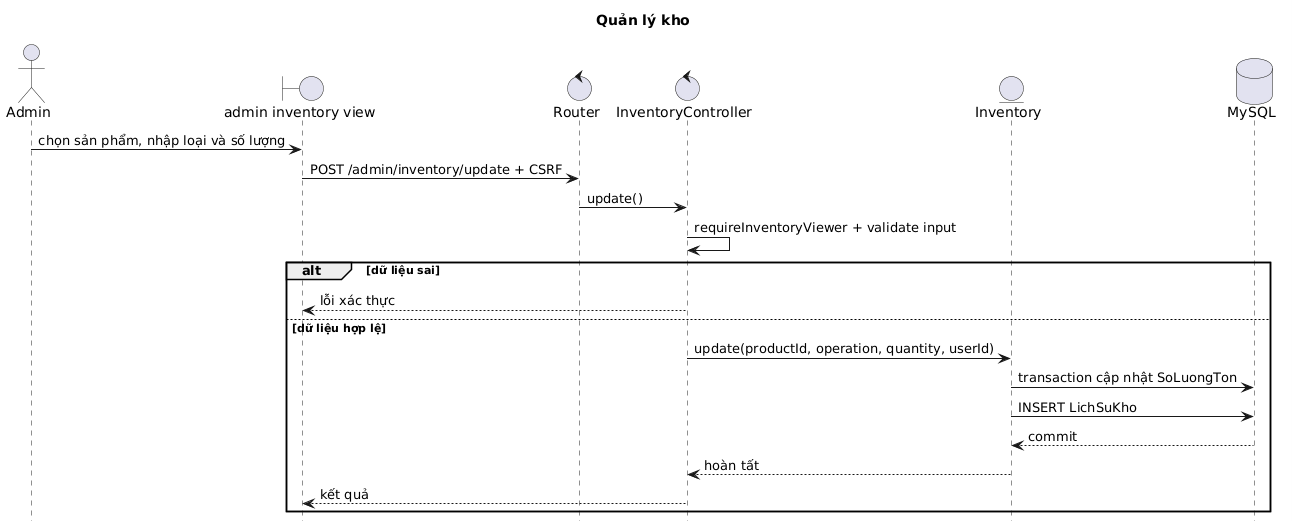
\includegraphics[width=0.9\textwidth, keepaspectratio]{Chapter_3/images_Usecase/qlykho.png}
    \caption{Sơ đồ trình tự Usecase Quản lý kho}
    \label{fig:uc-quan-ly-kho}
    \end{figure}

\section{UC15: Xem thống kê}
\begin{usecasetable}
    \textbf{Actor:} & Quản trị viên. \\ \hline
    \textbf{Mục tiêu:} & Cung cấp số liệu tổng quan phục vụ quản lý hoạt động kinh doanh. \\ \hline
    \textbf{Mô tả:} & Quản trị viên xem các số liệu về doanh thu, số lượng đơn hàng và tình hình sản phẩm theo khoảng thời gian được chọn. \\ \hline
    \textbf{Điều kiện trước:} & Quản trị viên đã đăng nhập. \\ \hline
    \textbf{Luồng chính:} & \begin{enumerate}
        \item Quản trị viên truy cập chức năng thống kê.
        \item Quản trị viên lựa chọn khoảng thời gian.
        \item Hệ thống tổng hợp dữ liệu liên quan.
        \item Hệ thống hiển thị kết quả thống kê.
    \end{enumerate} \\ \hline
    \textbf{Luồng thay thế / Ngoại lệ:} & Nếu khoảng thời gian không hợp lệ hoặc không có dữ liệu, hệ thống hiển thị thông báo phù hợp. \\ \hline
    \textbf{Điều kiện sau:} & Dữ liệu thống kê được hiển thị. \\ \hline
    \textbf{Quy tắc nghiệp vụ:} & \begin{itemize}
        \item Chỉ sử dụng dữ liệu hợp lệ hiện có trong hệ thống.
        \item Doanh thu chỉ được tính từ đơn hàng ở trạng thái Hoàn thành.
        \item Đơn hàng đã hủy hoặc chưa hoàn thành không được tính vào doanh thu thực tế.
    \end{itemize} \\ \hline
\end{usecasetable}

\section{UC16: Quản lý chương trình giảm giá}
\begin{usecasetable}
    \textbf{Actor:} & Quản trị viên. \\ \hline
    \textbf{Mục tiêu:} & Thiết lập và quản lý giá giảm cho sản phẩm trong một khoảng thời gian. \\ \hline
    \textbf{Mô tả:} & Quản trị viên tạo, chỉnh sửa, kích hoạt hoặc kết thúc chương trình giảm giá. Chương trình có thể áp dụng toàn trang hoặc chỉ cho một hoặc nhiều sản phẩm được chọn, với mức giảm theo phần trăm hoặc số tiền cố định. \\ \hline
    \textbf{Điều kiện trước:} & Quản trị viên đã đăng nhập và các sản phẩm mục tiêu đã tồn tại. \\ \hline
    \textbf{Luồng chính:} & \begin{enumerate}
        \item Quản trị viên truy cập chức năng quản lý chương trình giảm giá.
        \item Hệ thống hiển thị các chương trình và trạng thái hiện tại.
        \item Quản trị viên chọn tạo mới hoặc chỉnh sửa chương trình.
        \item Quản trị viên nhập tên, phạm vi, danh sách sản phẩm, loại và mức giảm, thời gian và trạng thái.
        \item Hệ thống kiểm tra dữ liệu, sản phẩm mục tiêu và thời hạn.
        \item Hệ thống lưu chương trình và xác định giá hiệu lực.
        \item Hệ thống hiển thị kết quả cập nhật.
    \end{enumerate} \\ \hline
    \textbf{Luồng thay thế / Ngoại lệ:} & \begin{itemize}
        \item Nếu mức giảm không hợp lệ, thời gian kết thúc không sau thời gian bắt đầu hoặc sản phẩm không tồn tại, hệ thống từ chối lưu.
        \item Nếu chương trình chưa bắt đầu, đã hết hạn hoặc bị tắt, hệ thống không áp dụng.
        \item Nếu nhiều chương trình cùng đủ điều kiện, hệ thống áp dụng mức giảm lớn nhất và không cộng dồn.
    \end{itemize} \\ \hline
    \textbf{Điều kiện sau:} & Chương trình được lưu; giá khuyến mãi chỉ có hiệu lực với sản phẩm và thời điểm thỏa điều kiện. \\ \hline
    \textbf{Quy tắc nghiệp vụ:} & \begin{itemize}
        \item Giá niêm yết được giữ nguyên; giá sau giảm không thấp hơn 0.
        \item Chương trình toàn trang áp dụng cho sản phẩm đang kinh doanh; chương trình cục bộ chỉ áp dụng cho sản phẩm được chỉ định.
        \item Thẻ sản phẩm, trang chi tiết, giỏ hàng và đặt hàng phải sử dụng cùng giá hiệu lực.
        \item Chỉnh sửa hoặc kết thúc chương trình không làm thay đổi giá đã được lưu trong đơn hàng đã tạo.
    \end{itemize} \\ \hline
\end{usecasetable}

\section{UC17: Quản lý voucher}
\begin{usecasetable}
    \textbf{Actor:} & Quản trị viên. \\ \hline
    \textbf{Mục tiêu:} & Tạo và kiểm soát mã ưu đãi do khách hàng chủ động nhập khi đặt hàng. \\ \hline
    \textbf{Mô tả:} & Quản trị viên tạo, chỉnh sửa, kích hoạt hoặc vô hiệu hóa voucher. Voucher có mã duy nhất, loại và mức giảm, thời hạn, giá trị đơn tối thiểu, mức giảm tối đa nếu là phần trăm, tổng lượt sử dụng và giới hạn theo khách hàng. \\ \hline
    \textbf{Điều kiện trước:} & Quản trị viên đã đăng nhập. \\ \hline
    \textbf{Luồng chính:} & \begin{enumerate}
        \item Quản trị viên mở chức năng quản lý voucher.
        \item Hệ thống hiển thị danh sách voucher và tình trạng sử dụng.
        \item Quản trị viên chọn tạo mới hoặc chỉnh sửa voucher.
        \item Quản trị viên nhập mã, mức giảm, điều kiện đơn hàng, thời hạn và giới hạn sử dụng.
        \item Hệ thống kiểm tra tính duy nhất của mã và tính hợp lệ của điều kiện.
        \item Hệ thống lưu voucher và thông báo kết quả.
    \end{enumerate} \\ \hline
    \textbf{Luồng thay thế / Ngoại lệ:} & Nếu mã bị trùng, mức giảm hoặc giới hạn không hợp lệ, hệ thống không lưu thay đổi. \\ \hline
    \textbf{Điều kiện sau:} & Voucher hợp lệ được lưu và có thể được khách hàng sử dụng trong thời hạn cho phép. \\ \hline
    \textbf{Quy tắc nghiệp vụ:} & \begin{itemize}
        \item Voucher bị tắt, chưa bắt đầu, hết hạn hoặc hết lượt không được áp dụng.
        \item Một đơn hàng chỉ sử dụng tối đa một voucher.
        \item Voucher được áp dụng sau chương trình giảm giá sản phẩm.
        \item Tổng tiền sau giảm không được âm và lượt sử dụng chỉ ghi nhận khi đơn được tạo thành công.
    \end{itemize} \\ \hline
\end{usecasetable}

\section{UC18: Áp dụng voucher khi đặt hàng}
\begin{usecasetable}
    \textbf{Actor:} & Khách hàng. \\ \hline
    \textbf{Mục tiêu:} & Sử dụng mã voucher hợp lệ để giảm số tiền phải trả cho đơn hàng. \\ \hline
    \textbf{Mô tả:} & Khách hàng nhập mã voucher ở bước kiểm tra đơn hàng. Hệ thống xác thực theo thời hạn, trạng thái, giá trị đơn, lượt sử dụng và điều kiện theo khách hàng trước khi tính lại tổng tiền. \\ \hline
    \textbf{Điều kiện trước:} & Khách hàng đã đăng nhập, giỏ hàng có sản phẩm và đang thực hiện UC05 -- Đặt hàng. \\ \hline
    \textbf{Luồng chính:} & \begin{enumerate}
        \item Khách hàng nhập mã voucher và yêu cầu áp dụng.
        \item Hệ thống chuẩn hóa mã và tìm voucher tương ứng.
        \item Hệ thống kiểm tra trạng thái, thời hạn, giá trị đơn tối thiểu, lượt sử dụng và điều kiện khách hàng.
        \item Hệ thống tính mức giảm trên tổng tiền sau khi đã áp dụng giảm giá sản phẩm.
        \item Hệ thống hiển thị mã áp dụng, số tiền giảm và tổng tiền mới.
        \item Khi khách hàng xác nhận đặt hàng, hệ thống kiểm tra lại điều kiện và ghi nhận lượt sử dụng cùng giao dịch tạo đơn.
    \end{enumerate} \\ \hline
    \textbf{Luồng thay thế / Ngoại lệ:} & \begin{itemize}
        \item Nếu mã không tồn tại, hết hạn, bị vô hiệu hóa, hết lượt hoặc không đủ điều kiện, hệ thống không giảm giá.
        \item Nếu giỏ hàng thay đổi khiến không đủ điều kiện, hệ thống tính lại tổng tiền.
        \item Nếu voucher hết lượt trước khi tạo đơn, hệ thống không ghi nhận voucher và yêu cầu xác nhận đơn với số tiền cập nhật.
    \end{itemize} \\ \hline
    \textbf{Điều kiện sau:} & Voucher hợp lệ được lưu cùng thông tin giảm giá thực tế của đơn hàng; voucher không hợp lệ không làm thay đổi tổng tiền. \\ \hline
    \textbf{Quy tắc nghiệp vụ:} & \begin{itemize}
        \item Trình duyệt không được quyết định số tiền giảm; hệ thống tự tính lại khi áp dụng và tạo đơn.
        \item Mã voucher và số tiền giảm thực tế phải được lưu trong đơn hàng.
        \item Chỉ tạo đơn thành công mới ghi nhận lượt sử dụng voucher.
    \end{itemize} \\ \hline
\end{usecasetable}
